\chapter{Introduction}\label{chap:introduction}
\section{Statistical Fault Localization}
Typical Statistical Fault Localization (SFL) techniques take data characterizing a set of both passing and failing program executions, including PASS/FAIL labels (provided by testers or end users) and recorded profiles of internal program dynamics, and they compute statistical measures of the strength of the association, if any, between the occurrence of software failures and the occurrence of certain runtime events at particular program locations.  These measures are then used to help guide the search for the causes of observed failures, typically by ranking program statements by the strengths of their associations with failures.  When SFL techniques are evaluated they are generally used as the sole source of information about possible fault locations.  However, it seems more realistic to envision them ultimately being used in combination with other sources of information, such as programmer hunches and {\it fault prediction models} \cite{Fenton1999} based on static code properties and project history.  Potentially, SFL techniques provide a relatively inexpensive way to maximize the information obtained by testing.


\section{Bugs in Numerical Software}
Numerical software plays a very important role in science, industry, and defense, and failures of numerical software have been reported as the cause of several well-publicized ``disasters" cite{VuikWeb,Kanewala2014}.  However, automated techniques intended specifically for localizing numerical faults based on execution data have received relatively little attention from researchers, although there has been substantial research on general {\it statistical fault localization} (SFL) techniques (e.g. \cite{Jones2002,Liblit2004,Liu2005}) and on other general automated debugging techniques (see Section 3.6).

Numerical bugs in the software are often hard to detect because they may not necessarily result in software crashes. It is very difficult to localize the fault by interrupting the execution (e.g. setting a breakpoint) and inspecting the value of intermediate variables, because we lack the oracle of intermediate variable values. Testers usually detect failures in numerical programs by checking whether the difference between the program output and expected output exceeds a pre-defined tolerance \cite{commontest}.

\section{Causal Inference with Statistical Fault Localization}
Coverage-based statistical fault localization (SFL) techniques apply statistical or machine learning techniques to code-coverage profiles (or ``spectra") and PASS/FAIL labels for a set of observed program executions, in order to identify possible locations of the fault(s) that caused some of the executions to fail.  These techniques equate the ``suspiciousness" of a program element with a statistical measure of the association between coverage of that element and the occurrence of program failures.  For example Baah et al showed \cite{baah2010causal} that the Tarantula metric \cite{jones2002visualization}, the Ochiai metric \cite{abreu2007accuracy}, and the F1-measure \cite{baah2010causal} each embed an estimator of the conditional probability of program failure given that a statement  is covered, which we denote by $P(F|s)$.  

It should be noted, first of all, that these and other suspiciousness metrics do {\it not} directly estimate the probability that a statement $s$ is {\it faulty}, because doing so would require data about observed faults, not just data about {\it failures}.  One might hope instead that such suspiciousness metrics yield good estimates of the {\it average causal effect} \cite{pearl2000models} of executing a given program element on the occurrence of failures, which we shall call the {\it average failure-causing effect} (AFCE).  Average causal effect estimates are used to study causality in a variety of fields, such as epidemiology, econometrics, and social science.  However, as Baah et al pointed out \cite{baah2010causal}, SFL suspiciousness metrics often produce biased estimates of a program element’s AFCE, due to the effects of other program elements.  For example, Figure \ref{fig2.1} shows a small function that contains a bug in statement $s_3$, which should be $y=x+2$.  Appropriately, $P(F|s_3)=1$.  However, because the faulty statement $s_3$ is always executed before either of the correct statements $s_5$ or $s_8$ is executed, $P(F|s_5)=P(F|s_8)=1$, which suggests misleadingly that $s_5$ and $s_8$ are faulty.

\begin{figure}[htb!]
\vspace{0em}
\begin{center}
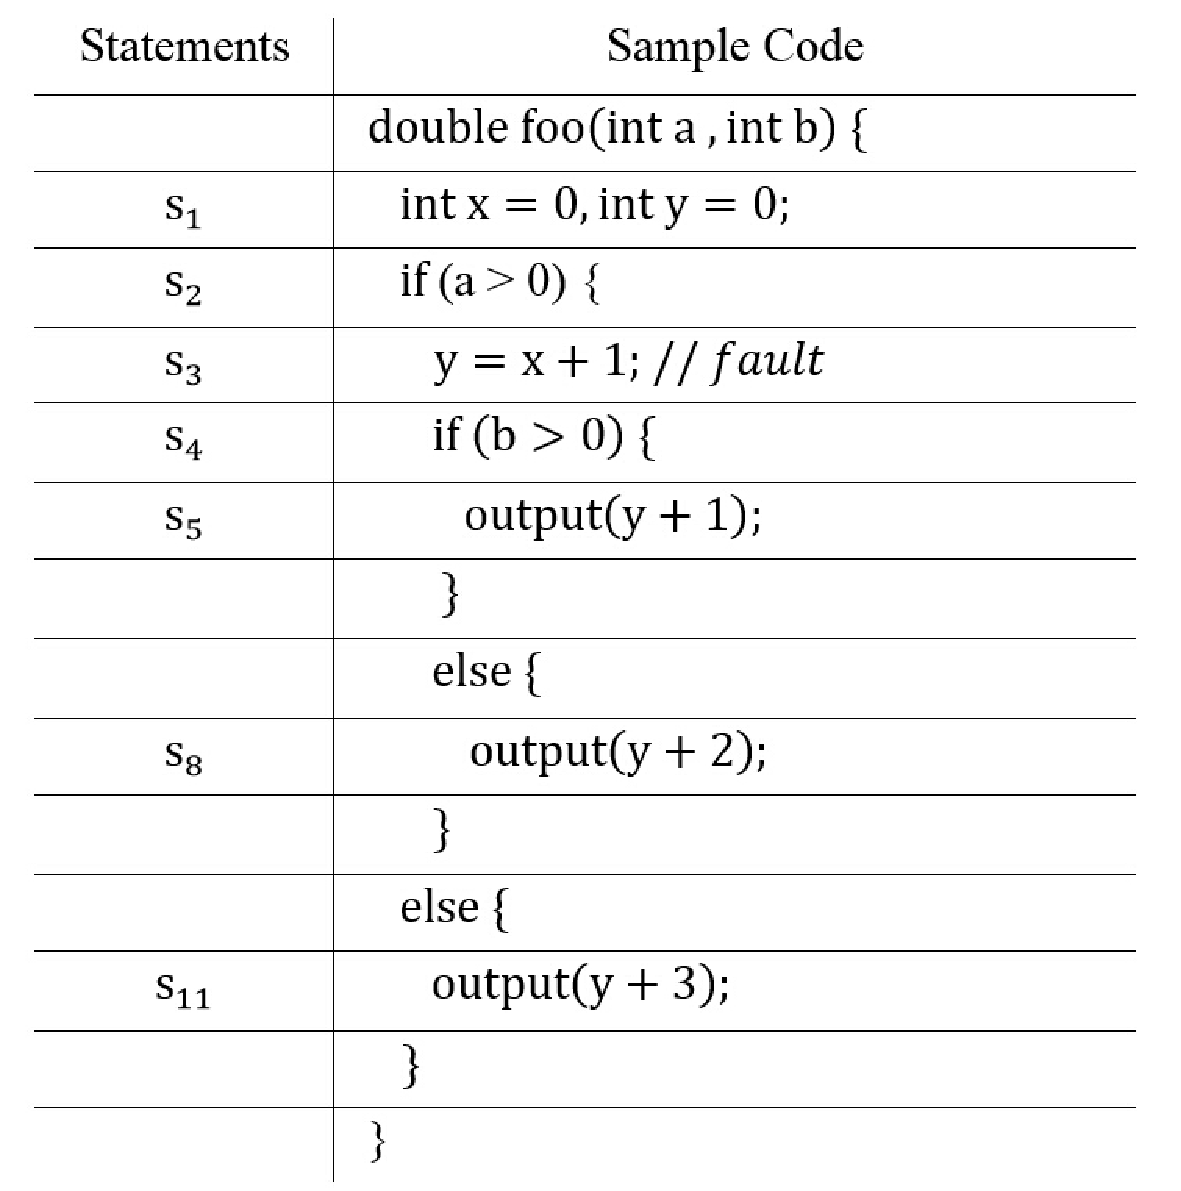
\includegraphics[width=0.6\textwidth]{chapter2_fig1.pdf}
\vspace {0em}\caption{Motivating Example} \label{fig2.1}
\end{center}
\vspace {0em}
\end{figure}

This problem, which is an instance of {\it confounding bias} (or just {\it confounding}) \cite{pearl2000models}, is due to the fact that execution of the control dependence region \cite{ball1993s} containing statements $s_3$ and $s_4$ is a {\it common cause} of program failure and of execution of statement $s_5$ or $s_8$.  More generally, confounding of the effect of a ``treatment" variable $T$ on an outcome variable $Y$ is bias due to the presence of a common cause $C$ of $T$ and $Y$.  Confounding bias cannot be eliminated, in general, without considering the causal relationships between the variables under study.  These relationships are typically represented in a {\it causal} DAG \cite{pearl2000models}, which is a directed acyclic graph in which there is an edge $A \rightarrow B$ just in case variable $A$ is a direct cause of variable $B$.  For example, Figure \ref{fig2.2} is a very simple causal graph showing the causal relationships between a treatment $T$, an outcome $Y$, and a confounder $C$.  For SFL, Baah et al \cite{baah2010causal,baah2011mitigating} proposed using a causal DAG derived from the {\it program dependence graph} (PDG) \cite{ferrante1987program}, in which the nodes represent binary coverage indicator variables.

Confounding can be reduced or eliminated by adjusting or controlling for a suitable set of variables during statistical analysis.  A well-known result of Pearl, the {\it Back-Door Adjustment Theorem} \cite{pearl2000models}, states that a set of covariates $\mathbf{X}$ in a causal DAG $G$ is sufficient for confounding adjustment if it ``blocks" all ``backdoor paths" between the treatment $T$ and the outcome $Y$.  A {\it backdoor path} between $T$ and $Y$ is a path with an arrow $T \leftarrow$ entering $T$.  A path is {\it blocked} by $\pmb{X}$ if the path (1) contains a configuration of the form $\rightarrow Z \rightarrow$ or $\leftarrow Z \rightarrow$ such that  $Z \in \mathbf{X}$ or (2) contains a ``collider" $\rightarrow Z \leftarrow$  such that neither $Z$ nor any of its descendants is in $\mathbf{X}$.  For example, in Figure \ref{fig2.2} the path $T \leftarrow C \rightarrow Y$ is a backdoor path, which is blocked by $C$.

\begin{figure}[htb!]
\vspace{0em}
\begin{center}
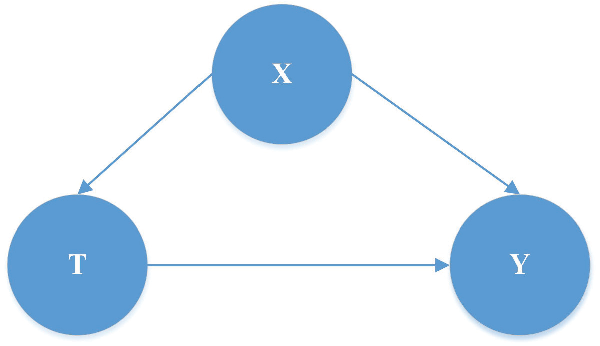
\includegraphics[width=0.6\textwidth]{chapter2_CausalDAG1.pdf}
\vspace {0em}\caption{Causal Diagram of treatment, outcome and confounder} \label{fig2.2}
\end{center}
\vspace {0em}
\end{figure}

\section{Contribution and Organization of The Dissertation}

This dissertation makes the following contributions: a novel value based approach to to SFL for numerical programs; an analysis of two types of violations of positivity - structural violations and random violations in casual fault localization; the first use of the Bayesian Additve Regression Tree  model to estimate failure-causing effects of numerical expressions.

The remainder of the dissertation is organized as follows:

Chapter 2 investigates the performance of Baah et al’s causal regression model for fault localization when the positivity condition is violated.

Chapter 3 presents NUMFL, which is a value based causal inference model for localizing faults in numerical softwares. NUMFL uses generalized propensity scores to control confounding bias.

Chapter 4 presents a new fault localization method, which is based on  the Bayesian Additive Regression Tree model.

Chapter 5 presents FLECS2.0, which is an approach to automatically localize faulty statements in embedded control softwares.

Chapter 6 concludes this dissertation and discusses possible improvements of proposed methods for future work.



